\newpage
\section{Resultados}

\newcommand{\graficoreservado}[3]{%
\begin{figure}[H]
    \centering
    \caption{#1}
    \label{#2}
    \vspace{0.3cm}
    \fbox{\parbox[c][4.2cm][c]{0.85\textwidth}{\centering Espaço reservado para o gráfico\\ #3}}
    \vspace{0.2cm} \\
    Fonte: Autor.
\end{figure}}

\par Este capítulo apresenta os resultados obtidos com o sistema desenvolvido e discute até que ponto eles confirmam os requisitos especificados. Conforme a estrutura apresentada na introdução, a avaliação combina três fontes de evidência: as medidas de desempenho feitas com o sistema completo em contêineres, o ensaio de aquisição contra um servidor Modbus TCP de teste e os ensaios na bancada com o inversor de frequência. Primeiro, descreve-se o ambiente em que as medidas foram feitas e o método comum a todas elas. Em seguida, são apresentadas as medidas já realizadas, que cobrem o cadastro de clientes, a autenticação, o tempo de resposta das telas, o motor de scripts isolado e a gravação do histórico. Depois, relata-se a capacidade de aquisição, medida com simuladores, e o ensaio ponta a ponta contra o servidor de teste. Na sequência, reservam-se os espaços para os seis ensaios da bancada, com o comportamento esperado em cada um. Por fim, os requisitos são confrontados com as evidências, resume-se a qualidade de software e discutem-se as limitações observadas e a relação dos resultados com a literatura.

\subsection{Ambiente de ensaio}

\par As medidas foram obtidas em um único computador, o do próprio autor, que fez o papel de servidor. Todos os processos do sistema executaram em contêineres \emph{Docker} \cite{DOCKER_DOCS}, cada um com limites de processamento e de memória definidos para reproduzir os recursos planejados para a implantação, de modo que o teto medido seja o de um contêiner pequeno e não o da máquina inteira. O \emph{PostgreSQL} \cite{POSTGRESQL_DOCS} na versão 18 e o \emph{Redis} \cite{REDIS_DOCS} na versão 8 também executaram em contêineres. A Tabela~\ref{tab:cap7_ambiente} resume o equipamento e as versões, e a Tabela~\ref{tab:cap7_limites} lista os limites aplicados a cada contêiner.

{\renewcommand{\arraystretch}{1.3}\small
\begin{xltabular}{\textwidth}{lX}
        \caption{Ambiente de ensaio.}
        \label{tab:cap7_ambiente}\\
        \hline
        \textbf{Item} & \textbf{Descrição} \\
        \hline
        \endfirsthead
        \hline
        \textbf{Item} & \textbf{Descrição} \\
        \hline
        \endhead
        \endfoot
        \multicolumn{2}{c}{Fonte: Autor.} \\
        \endlastfoot
        Computador (servidor) & Intel Core i5-13420H com 12 \emph{threads}, cerca de 32\,GB de memória, Windows 11 Pro \\
        \hline
        Virtualização & Docker Desktop com máquina virtual de 4 processadores lógicos e 6\,GB de memória durante a campanha de capacidade \\
        \hline
        Banco de dados & PostgreSQL 18.6 em contêiner \\
        \hline
        Cache, filas e transporte & Redis 8.10 em contêiner, com política \emph{noeviction} \\
        \hline
        Aplicação & Node.js 24, imagens de produção construídas em estágios, uma por serviço \\
        \hline
        Dispositivo de campo simulado & Simuladores Modbus TCP, um do próprio repositório, com milhares de \sigla{clp} virtuais, e o ProtoProbe do autor (porta 502, escravo 1) \\
        \hline
        Arquitetura do processador & amd64 no ensaio, enquanto a implantação prevê processadores ARM \\
        \hline
\end{xltabular}}

{\renewcommand{\arraystretch}{1.3}\small
\begin{xltabular}{\textwidth}{lccX}
        \caption{Limites de recursos dos contêineres.}
        \label{tab:cap7_limites}\\
        \hline
        \textbf{Contêiner} & \textbf{Processamento} & \textbf{Memória} & \textbf{Observação} \\
        \hline
        \endfirsthead
        \hline
        \textbf{Contêiner} & \textbf{Processamento} & \textbf{Memória} & \textbf{Observação} \\
        \hline
        \endhead
        \endfoot
        \multicolumn{4}{c}{Fonte: Autor.} \\
        \endlastfoot
        API (Fastify) & 0,25 \emph{vCPU} & 512\,MB & Processo HTTP, sem \emph{workers} \\
        \hline
        \emph{Worker} & 0,25 \emph{vCPU} & 512\,MB & Um supervisor e um subprocesso por família de fila \\
        \hline
        Aquisição & 0,25 \emph{vCPU} & 512\,MB & Agendador e leitura Modbus, sem banco \\
        \hline
        Scripts isolados & 0,25 \emph{vCPU} & 512\,MB & Hospedeiro do \emph{WebAssembly}, raiz somente leitura \\
        \hline
        Web (Next.js) & 0,25 \emph{vCPU} & 512\,MB & Somente telas \\
        \hline
        Redis & 0,25 \emph{vCPU} & 1\,GB & \emph{maxmemory} de 512\,MB \\
        \hline
        PostgreSQL & 2 \emph{vCPU} & 1\,GB & \emph{shared\_buffers} de 256\,MB \\
        \hline
\end{xltabular}}

\par A soma dos limites é de 3,5 \emph{vCPU} e 4,5\,GiB, que cabe na máquina virtual usada. Os limites de processamento são aplicados por cota de tempo, o mesmo mecanismo usado pelos orquestradores de contêineres, o que faz um contêiner de 0,25 \emph{vCPU} parar por alguns milissegundos ao esgotar a cota em cada janela de tempo. Esse comportamento aparece nos resultados, por exemplo no percentil 95 da latência do motor de scripts, e é uma característica do ambiente e não do código.

\par O método dos ensaios de capacidade foi o mesmo em todos os tipos de carga. Cada degrau de carga roda dois ciclos de aquecimento, descartados, e doze ciclos medidos. Um degrau é considerado sustentado quando pelo menos 99\,\% das leituras esperadas foram atendidas, o atraso no percentil 95 ficou abaixo de 20\,\% do período de varredura, a profundidade das filas não cresceu na segunda metade da janela, nenhum contêiner reiniciou e o Redis ficou abaixo de 70\,\% da memória máxima configurada. O teto de um tipo de carga é o maior degrau sustentado antes do primeiro reprovado, e um degrau reprovado que passa ao ser repetido é tratado como ruído de medição. Esse critério acompanha a prática das avaliações experimentais da literatura de contêineres, que mede latência, vazão e consumo de processador e de memória sob carga crescente \cite{NETTO2019_RAFT_KUBERNETES,NETTO2016_STATE_MACHINE_REPLICATION_KUBERNETES}.

\par Há ressalvas que valem para todos os resultados. A carga, o simulador de \sigla{clp}, o navegador e os contêineres dividem o mesmo computador, que também executava outras atividades do autor. Não há latência de rede entre os contêineres, nem balanceador, nem criptografia de transporte no Redis. O PostgreSQL local tem disco rápido e aceita muito mais conexões que a instância de 1\,GiB prevista. Os números, portanto, são de ordem de grandeza e valem como teto do servidor com equipamento que responde de imediato, e não como previsão para uma planta com modems lentos.

\subsection{Medidas de desempenho já realizadas}

\subsubsection{Cadastro de clientes e custo da autenticação}

\par O sistema é multi-tenant com banco próprio por cliente, e por isso a criação de um cliente envolve criar o banco, aplicar o esquema e cadastrar os dados iniciais, tudo num trabalho assíncrono retomável. Mediu-se o tempo entre o pedido de criação e o banco pronto para uso. Com o sistema aquecido, o processo levou 1,7 s e, na primeira criação de um cliente, que inclui o ensaio da migração com reversão, levou 3,4 s. O aplicador de migrações sozinho levou de 0,36 a 0,54 s. Esses valores sustentam o requisito de banco próprio por cliente, criado de forma automática (RF12), pois a entrada de um novo cliente não exige intervenção manual nem espera perceptível.

\par A exclusão de um cliente é a operação inversa e mais cara. O comando que remove o banco com desconexão forçada levou de 5 a 18 s na pilha local anterior, tempo dominado pelo ponto de verificação do banco. A limpeza das chaves do cliente no Redis usa uma varredura incremental cujo custo cresce com o total de chaves da instância e não com as chaves do cliente, com cerca de 15 ms para 500 chaves, de 0,08 a 0,37 s para 20 mil e de 0,56 a 1,4 s para 100 mil. Como a exclusão roda em segundo plano e não bloqueia as telas, esses tempos são aceitáveis, mas indicam que a limpeza deve ser repensada se o Redis for compartilhado por muitos clientes. Na campanha de capacidade, a exclusão de clientes de teste ficou em execução por horas sem terminar, achado registrado e ainda sem causa comprovada, o que a seção de limitações retoma.

\todo[inline]{Conferir se o achado da campanha de 13 e 14/10 (exclusão de cliente que não termina na pilha de capacidade) foi corrigido depois do relatório. O texto o trata como pendente.}

\par A autenticação usa o \emph{Argon2id}, função de derivação de chave projetada para dificultar ataques por força bruta com \emph{hardware} paralelo \cite{ARGON2_RFC9106}. Com 19.456\,KiB de memória, duas iterações e um nível de paralelismo, medido em 30 amostras no processador do ensaio, o cálculo do \emph{hash} teve mediana de 24,2 ms e percentil 95 de 26,2 ms, e a verificação teve mediana de 23,9 ms e percentil 95 de 26,8 ms. O custo é imperceptível para quem entra no sistema e, ao mesmo tempo, caro o bastante para tornar impraticável a tentativa em massa de senhas contra um banco vazado, o que atende ao requisito de segurança de acesso (RNF05). A Tabela~\ref{tab:cap7_infra} reúne essas medidas.

{\renewcommand{\arraystretch}{1.3}\small
\begin{xltabular}{\textwidth}{Xcc}
        \caption{Medidas de criação de cliente e de autenticação.}
        \label{tab:cap7_infra}\\
        \hline
        \textbf{Medida} & \textbf{Resultado} & \textbf{Data} \\
        \hline
        \endfirsthead
        \hline
        \textbf{Medida} & \textbf{Resultado} & \textbf{Data} \\
        \hline
        \endhead
        \endfoot
        \multicolumn{3}{c}{Fonte: Autor.} \\
        \endlastfoot
        Criação de cliente, pedido até banco pronto & 1,7 s (quente) e 3,4 s (frio) & 08/10/2026 \\
        \hline
        Aplicação das migrações do cliente & 0,36 a 0,54 s & 08/10/2026 \\
        \hline
        Remoção do banco do cliente (\emph{DROP DATABASE} forçado) & 5 a 18 s & 08/10/2026 \\
        \hline
        Limpeza de chaves do Redis, 500 e 100 mil chaves & 15 ms e de 0,56 a 1,4 s & 08/10/2026 \\
        \hline
        \emph{Hash} de senha Argon2id, mediana e percentil 95 & 24,2 ms e 26,2 ms & 08/10/2026 \\
        \hline
        Verificação de senha Argon2id, mediana e percentil 95 & 23,9 ms e 26,8 ms & 08/10/2026 \\
        \hline
\end{xltabular}}

\subsubsection{Desempenho das telas}

\par O desempenho das telas foi medido com o \emph{Lighthouse} em modo de celular, com limitação simulada de rede e de processador, sobre a versão de produção da interface e uma instância isolada do sistema, com a sessão de um usuário de teste. Foram feitas três execuções em cada uma das três telas principais, o sinótico em modo de execução, a lista de alarmes e o dashboard, e a Tabela~\ref{tab:cap7_lighthouse} apresenta a mediana, junto com o piso adotado como limite de regressão para os próximos lotes. O \emph{Largest Contentful Paint}, que mede o tempo até o maior elemento aparecer, ficou entre 1,25 e 1,51 s, abaixo do alvo de 2,5 s, e o deslocamento de \emph{layout} acumulado ficou muito abaixo do limite de 0,1. O tempo total de bloqueio da \emph{thread} principal, que serve de aproximação da responsividade, foi maior no dashboard por causa do desenho dos gráficos.

{\renewcommand{\arraystretch}{1.3}\small
\begin{xltabular}{\textwidth}{Xccccccc}
        \caption{Resultados do \emph{Lighthouse} (celular), mediana de três execuções. Des.: desempenho, Ace.: acessibilidade, BP: boas práticas, LCP e TBT em ms.}
        \label{tab:cap7_lighthouse}\\
        \hline
        \textbf{Tela} & \textbf{Des.} & \textbf{Ace.} & \textbf{BP} & \textbf{SEO} & \textbf{LCP} & \textbf{CLS} & \textbf{TBT} \\
        \hline
        \endfirsthead
        \hline
        \textbf{Tela} & \textbf{Des.} & \textbf{Ace.} & \textbf{BP} & \textbf{SEO} & \textbf{LCP} & \textbf{CLS} & \textbf{TBT} \\
        \hline
        \endhead
        \endfoot
        \multicolumn{8}{c}{Fonte: Autor.} \\
        \endlastfoot
        Sinótico (execução) & 99 & 100 & 100 & 54 & 1.260 & 0 & 121 \\
        \hline
        Alarmes & 99 & 100 & 100 & 54 & 1.253 & 0,008 & 141 \\
        \hline
        Dashboard & 94 & 100 & 100 & 54 & 1.513 & 0,001 & 282 \\
        \hline
        Piso adotado & 94 / 94 / 89 & 95 & 95 & 49 & - & - & - \\
        \hline
\end{xltabular}}

\par A pontuação de acessibilidade em 100 indica que o teste automático não encontrou violação das diretrizes \sigla{wcag}, o que não substitui a conferência com leitor de tela e com a navegação por teclado, que ficou como risco aceito. A pontuação de \emph{SEO} em 54 é esperada e não representa defeito, porque a área autenticada é marcada como não indexável por decisão de projeto. A medição foi feita com outras atividades pesadas no mesmo computador, de modo que os valores tendem a ser conservadores. As medidas dão suporte ao requisito de acesso por navegador sem instalação (RNF13) e ao de exibição das telas de supervisão (RF15 e RF16).

\todo[inline]{As medianas vêm do registro de 15/10/2026 (madrugada) e o piso consta no CLAUDE.md do código com data de 14/10/2026. Confirmar qual data deve aparecer no texto e se vale citar o INP, que o Lighthouse não mede em modo de navegação.}

\par Além da pontuação geral, mediu-se o custo de atualizar uma tela de sinótico com muitos objetos. Uma tela de teste com 200 objetos, 120 vínculos entre objetos e tags e 506 nós gráficos foi mantida aberta por 60 s com dez tags que mudavam a cada ciclo. Nenhuma tarefa longa, isto é, nenhuma tarefa de mais de 50 ms na \emph{thread} principal, foi registrada. O tempo para aplicar um ciclo de valores, medido do fim da resposta até a última alteração na árvore da página, teve mediana de 6 ms e percentil 95 de 8 ms, abaixo do orçamento de 16 ms, que corresponde a um quadro de uma tela de 60 quadros por segundo. Esse resultado mostra que o ritmo de atualização por \emph{polling} curto não degrada a interface e sustenta, do lado do cliente, o requisito de telas de tempo real com baixa latência (RNF01) e o de execução do sinótico (RF16).

\subsubsection{Motor de scripts isolado}

\par O cálculo de variáveis derivadas, de scripts de eventos e de componentes de conteúdo escritos pelos clientes executa em um motor isolado, com o interpretador \emph{QuickJS} \cite{QUICKJS_DOCS} compilado para \emph{WebAssembly} \cite{WEBASSEMBLY_SPEC} e executado sob o \emph{Wasmtime} \cite{WASMTIME_DOCS}, sem acesso a rede, arquivo, banco nem segredo. O isolamento, exigido pelo requisito de execução segura do código do usuário (RNF07), tem um custo, e as medidas procuram dimensioná-lo. Com um hospedeiro já aquecido em um contêiner de 0,25 \emph{vCPU}, o custo fixo de uma avaliação foi de 3,1 ms na mediana para a variável derivada, 3,5 ms para o script e 3,3 ms para o componente. O percentil 95 ficou entre 46 e 56 ms e o 99 entre 58 e 60 ms. Esses valores altos nas caudas correspondem à pausa da cota de processador, e não ao motor. O motor anterior, em \emph{Python}, custava cerca de 34 ms por avaliação nas mesmas condições, o que justificou a troca.

\par A vazão foi medida com um programa de comparação que executa avaliações em sequência. Um hospedeiro de 0,25 \emph{vCPU} sustentou de 144 a 149 avaliações por segundo, e quatro hospedeiros chegaram a 353. Por \emph{vCPU}, isso equivale a uma faixa de 380 a 590 avaliações por segundo, com ruído de cerca de 50\,\% entre execuções, porque o computador do ensaio executava outras cargas. O agrupamento de avaliações em lote aumentou a vazão, como mostra a Figura~\ref{fig:cap7_lote}. Com lote de 25 avaliações, o mesmo hospedeiro chegou, em média, a 545 avaliações por segundo, cerca de 3,7 vezes a de uma avaliação por vez.

\begin{figure}[H]
    \centering
    \caption{Vazão do motor de scripts em função do tamanho do lote, um hospedeiro de 0,25 \emph{vCPU}.}
    \label{fig:cap7_lote}
    \vspace{0.4cm}
    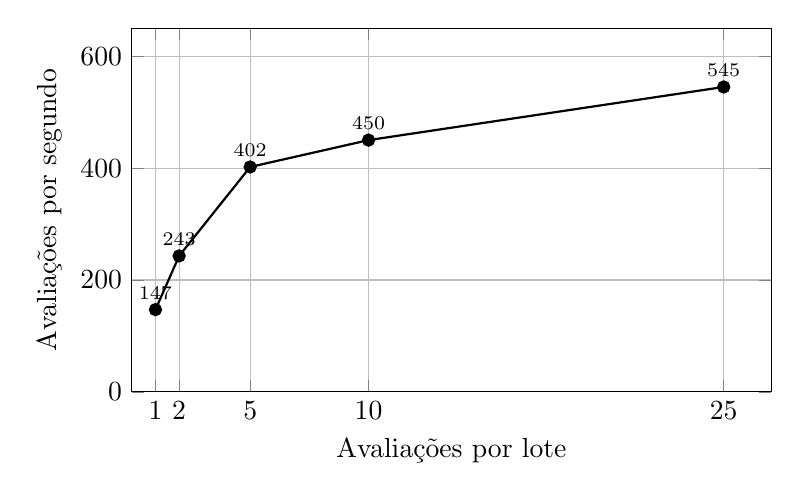
\begin{tikzpicture}
        \begin{axis}[
            width=0.8\textwidth, height=6.2cm,
            xlabel={Avaliações por lote},
            ylabel={Avaliações por segundo},
            xmin=0, xmax=27, ymin=0, ymax=650,
            xtick={1,2,5,10,25},
            grid=major,
            nodes near coords,
            every node near coord/.append style={font=\scriptsize, anchor=south},
        ]
            \addplot[mark=*, thick] coordinates {(1,147) (2,243) (5,402) (10,450) (25,545)};
        \end{axis}
    \end{tikzpicture}
    \vspace{0.2cm} \\
    Fonte: Autor.
\end{figure}

\par O ponto de maior interesse é o comportamento com muitos clientes ativos. Cada troca de cliente em um hospedeiro obriga a reciclar o ambiente de execução, para que nada de um cliente vaze ao seguinte, e essa reciclagem custa cerca de 0,55 s a 0,25 \emph{vCPU}, quase 180 vezes o custo de uma avaliação. Com três hospedeiros, um cliente ativo usou 121 avaliações por segundo, três clientes ativos chegaram a 253, que é 74\,\% do ideal de 340, e seis ou mais clientes derrubaram a vazão para menos de duas avaliações por segundo, como mostra a Figura~\ref{fig:cap7_clientes}. A conclusão de projeto é que o número de clientes ativos por contêiner não deve passar o número de hospedeiros, e que a escala se faz por réplicas do contêiner. O resultado ilustra o compromisso entre isolamento forte e desempenho, e só se torna problema quando muitos clientes avaliam scripts simultaneamente, o que o agrupamento por cliente atenua na prática. Essas medidas confirmam o requisito de cálculo de valores derivados e de execução de scripts (RF13 e RF14) e mostram o seu custo em recursos.

\begin{figure}[H]
    \centering
    \caption{Vazão do motor de scripts com três hospedeiros em função do número de clientes ativos.}
    \label{fig:cap7_clientes}
    \vspace{0.4cm}
    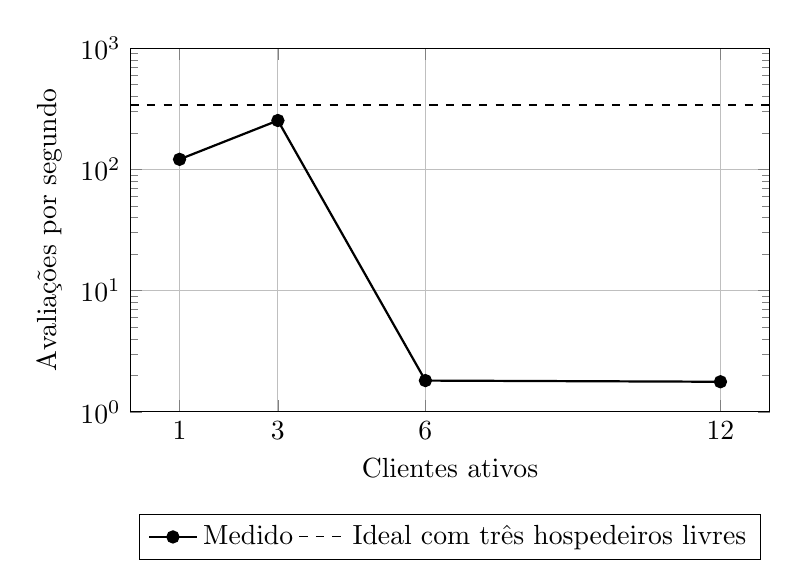
\begin{tikzpicture}
        \begin{axis}[
            width=0.8\textwidth, height=6.2cm,
            xlabel={Clientes ativos},
            ylabel={Avaliações por segundo},
            ymode=log, xmin=0, xmax=13, ymin=1, ymax=1000,
            xtick={1,3,6,12},
            grid=major,
            legend style={at={(0.5,-0.28)}, anchor=north, legend columns=2},
        ]
            \addplot[mark=*, thick] coordinates {(1,121) (3,253) (6,1.81) (12,1.77)};
            \addplot[dashed, domain=0:13] {340};
            \legend{Medido, Ideal com três hospedeiros livres}
        \end{axis}
    \end{tikzpicture}
    \vspace{0.2cm} \\
    Fonte: Autor.
\end{figure}

\par Quanto à memória, o hospedeiro do motor usou 17\,MiB de memória residente no teste de vazão, e o contêiner dedicado aos scripts atingiu o pico de 166\,MiB dos 512\,MiB permitidos. No contêiner de \emph{workers}, que concentra a ingestão e o histórico, o pico foi de 435\,MiB, ou 85\,\% do limite, o mais apertado de todos, e a API chegou a 340\,MiB. Esses números mostram que o isolamento dos scripts é barato em memória e que o limite que merece atenção é o do \emph{worker}.

\par A Tabela~\ref{tab:cap7_meta} traz o teto sustentado de variáveis derivadas, chamadas de metas, e de tags internas geradas, comparado com o piso planejado. As variáveis derivadas usadas no ensaio liam duas tags e foram avaliadas de 1,2 a 1,85 vezes por ciclo. As tags internas foram geradas em lotes de 25 por dispositivo. Em todos os casos, o primeiro recurso a saturar foi o contêiner de \emph{workers}, nas filas de ingestão e de histórico, e não o motor de scripts, que consome 3 ms por avaliação. As metas ficaram abaixo do piso planejado a 5 e a 30 s e no piso a 10 s, e as tags internas ficaram abaixo do piso nas três faixas, o que levou à abertura de uma especificação dedicada à capacidade dessas duas filas.

{\renewcommand{\arraystretch}{1.3}\small
\begin{xltabular}{\textwidth}{lcccc}
        \caption{Teto sustentado de variáveis derivadas e de tags internas geradas por contêiner de 0,25 \emph{vCPU}.}
        \label{tab:cap7_meta}\\
        \hline
        \textbf{Carga} & \textbf{Período} & \textbf{Teto medido} & \textbf{Piso planejado} & \textbf{Alvo} \\
        \hline
        \endfirsthead
        \hline
        \textbf{Carga} & \textbf{Período} & \textbf{Teto medido} & \textbf{Piso planejado} & \textbf{Alvo} \\
        \hline
        \endhead
        \endfoot
        \multicolumn{5}{c}{Fonte: Autor.} \\
        \endlastfoot
        Variável derivada (meta) & 5 s & 50 & 150 & 450 \\
        \hline
        Variável derivada (meta) & 10 s & 250 & 250 & 750 \\
        \hline
        Variável derivada (meta) & 30 s & 150 & 1.000 & 3.000 \\
        \hline
        Tag interna gerada & 5 s & 100 & 350 & 1.050 \\
        \hline
        Tag interna gerada & 10 s & 350 & 525 & 1.575 \\
        \hline
        Tag interna gerada & 30 s & 250 & 2.800 & 8.400 \\
        \hline
\end{xltabular}}

\subsubsection{Gravação do histórico e isolamento entre clientes}

\par O histórico de leituras é gravado por uma fila dedicada, em lotes, com decisão atômica de gravar e gravação idempotente, numa tabela particionada por mês. O teste de carga dessa fila mediu, para um cliente, de 186 a 235 trabalhos por segundo com 40 linhas cada, o que equivale a 7.430 a 9.400 linhas por segundo, a um custo de 1,8 a 2,7 ms de processador por trabalho. Com quatro clientes simultâneos, a taxa ficou entre 128 e 277 trabalhos por segundo. A decisão de gravar, feita por um \emph{script} no Redis, custou 16,4 \textmu s por chamada e 2,3\,\% do processador do Redis a 1.000 leituras por segundo. A retirada de 200.000 linhas pelo expurgo levou 1,6 s, ou 125 mil linhas por segundo. Esses resultados sustentam o registro contínuo do histórico (RF02) com folga em relação à carga de um cliente típico.

\par O mesmo teste verifica se um cliente que gera muito trabalho prejudica os demais. Nos dois cenários de sobrecarga de um cliente lento, o de pressão alta e o de controle com pressão baixa, a latência máxima de gravação do cliente vizinho ficou, depois das correções, entre 274 e 426 ms no primeiro e entre 303 e 313 ms no segundo, contra o limite de 15 s do critério. Nas primeiras execuções, porém, o limite foi ultrapassado, com 20,2 s no cenário de pressão alta e com 54,9 e 77,3 s no de controle. A investigação mostrou que o cenário anterior deixava milhares de trabalhos na fila e contaminava o seguinte, o que foi corrigido no teste, e que o resultado é muito sensível à disputa de processador na máquina, pois com oito laços de processamento ocupando o computador a latência do vizinho foi de 91,8 s. O resultado confirma o enfileiramento justo entre clientes (RNF03) em condições normais e mostra uma fragilidade sob escassez de processador, hoje registrada como risco do projeto.

\par Outro teste de carga manteve, por 10 minutos, seis clientes com leituras contínuas e conferiu que nenhuma tag ficava desatualizada na leitura final. Depois de uma correção no próprio teste, que passou a considerar o catálogo já carregado, três execuções seguidas passaram, em 639, 652 e 636 s. Isso confirma que o valor atual das tags permanece disponível e atualizado no Redis sob carga contínua (RF03), e que o orçamento de conexões do banco impõe espera, e não perda, quando o número de clientes simultâneos excede o de conexões reservadas.

\subsection{Aquisição e ensaio com o simulador}

\subsubsection{Capacidade de leitura Modbus}

\par A capacidade de aquisição foi medida com um simulador Modbus TCP do próprio repositório, que emula milhares de \sigla{clp} virtuais em portas distintas e registra as requisições recebidas. Cada \sigla{clp} virtual tinha 25 tags, lidas em cinco requisições por ciclo, número que o planejador do sistema gera para blocos de registradores afastados. A Tabela~\ref{tab:cap7_aquisicao} resume o teto de uma única réplica do serviço de aquisição, com 0,25 \emph{vCPU}, em três períodos de varredura. O que limitou a carga foi a soma do processador da aquisição e do Redis, ambos próximos de 100\,\% do limite, e não o banco de dados, que tinha dois processadores. O teto em tags por segundo foi praticamente o mesmo em 10 e em 30 s, entre 250 e 325 tags por segundo, o que confirma que o limite é de capacidade de processamento e não do ciclo de varredura.

{\renewcommand{\arraystretch}{1.3}\small
\begin{xltabular}{\textwidth}{cXcc}
        \caption{Teto de leitura Modbus por réplica de aquisição (0,25 \emph{vCPU}, 25 tags por CLP, cinco requisições por ciclo).}
        \label{tab:cap7_aquisicao}\\
        \hline
        \textbf{Período} & \textbf{Reprovou em} & \textbf{Teto (tags)} & \textbf{Tags por segundo} \\
        \hline
        \endfirsthead
        \hline
        \textbf{Período} & \textbf{Reprovou em} & \textbf{Teto (tags)} & \textbf{Tags por segundo} \\
        \hline
        \endhead
        \endfoot
        \multicolumn{4}{c}{Fonte: Autor.} \\
        \endlastfoot
        5 s & 1.500 tags, atraso no percentil 95 de 1.052 ms (limite de 1.000 ms) & 1.250 & 250 \\
        \hline
        10 s & 4.000 tags, atraso no percentil 95 de 4.882 ms e fila de despacho crescendo & 3.250 & 325 \\
        \hline
        30 s & 12.200 tags, atraso no percentil 95 de 8.306 ms (limite de 6.000 ms) & 9.750 & 325 \\
        \hline
\end{xltabular}}

\par A Figura~\ref{fig:cap7_aquisicao} compara esses tetos com os obtidos em rodadas anteriores com uma única requisição por \sigla{clp} e ciclo. O custo da requisição é significativo, porque cada ida e volta Modbus tem um custo fixo de enquadramento, resposta e despacho independente do número de registradores. Passar de uma para cinco requisições reduziu o teto de 2.000 para 1.250 tags a 5 s, queda de 37\,\%, e de 4.000 para 3.250 a 10 s, queda de 19\,\%. Em equipamentos reais, o tempo de resposta do \emph{modem} e da rede soma-se a cada requisição, de modo que o teto prático será menor. A medida dimensiona uma réplica, mas o efeito de uma segunda réplica não foi medido, de modo que a replicação horizontal (RNF02) é sustentada pela arquitetura. O requisito de aquisição periódica (RF01) fica confirmado em carga. Como a fila reparte o trabalho e o Moleculer leva cada dispositivo sempre à mesma réplica, o total deve crescer com o número de réplicas até o Redis passar a ser o limite, o que também chegou perto de 100\,\% no ensaio.

\begin{figure}[H]
    \centering
    \caption{Teto de tags por réplica de aquisição, com uma e com cinco requisições por CLP.}
    \label{fig:cap7_aquisicao}
    \vspace{0.4cm}
    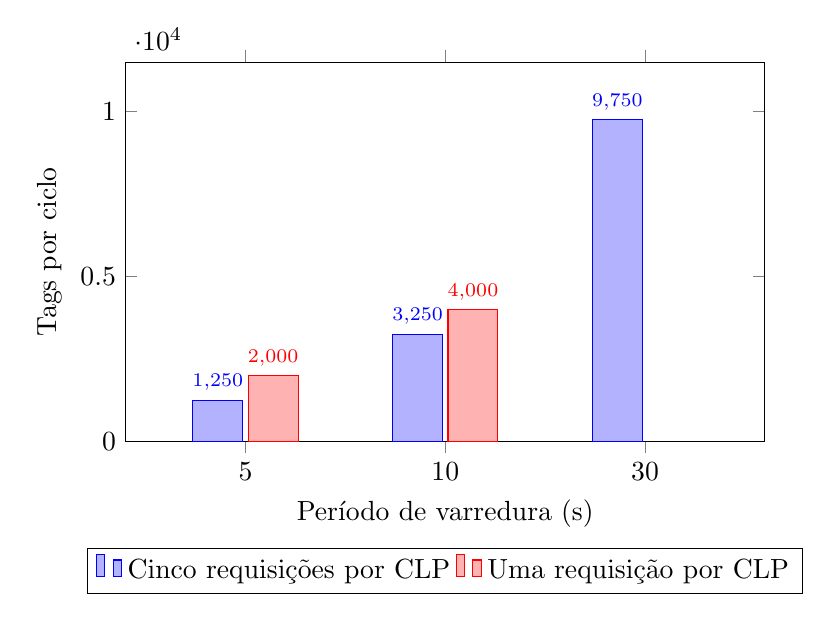
\begin{tikzpicture}
        \begin{axis}[
            ybar, width=0.8\textwidth, height=6.4cm,
            symbolic x coords={5,10,30},
            xtick=data,
            xlabel={Período de varredura (s)},
            ylabel={Tags por ciclo},
            ymin=0, ymax=11500, bar width=18pt, enlarge x limits=0.3,
            nodes near coords,
            every node near coord/.append style={font=\scriptsize},
            legend style={at={(0.5,-0.28)}, anchor=north, legend columns=2},
        ]
            \addplot coordinates {(5,1250) (10,3250) (30,9750)};
            \addplot coordinates {(5,2000) (10,4000)};
            \legend{Cinco requisições por CLP, Uma requisição por CLP}
        \end{axis}
    \end{tikzpicture}
    \vspace{0.2cm} \\
    Fonte: Autor.
\end{figure}

\subsubsection{Ensaio ponta a ponta com o servidor de teste}

\par Para validar a cadeia completa contra um servidor que se comporta como um \sigla{clp} comum, o autor usou o ProtoProbe, um servidor Modbus TCP de teste que escuta na porta 502 com identificador de escravo 1 e expõe 2.500 registradores de retenção de 16 bits sem sinal. O ensaio cadastrou, pela interface do sistema, uma planta, um dispositivo Modbus apontando para o servidor e uma tag no endereço 7, lida de 1 em 1 s com função de leitura de registradores de retenção. Também se cadastrou um dispositivo interno com uma tag gravável, um evento que compara a tag lida com um limite e um \emph{script} que copia o valor lido para a tag interna. Nenhuma função de escrita foi usada nessa prova.

\par O resultado foi positivo em toda a cadeia. O valor 12.314, que o servidor de teste mantém no endereço 7, chegou ao valor atual da tag com qualidade boa. O evento disparou, o \emph{script} executou no contêiner isolado em 13 a 87 ms e gravou a tag interna com o mesmo valor, sem falha registrada. Como os registradores do servidor de teste são estáticos, o limite do evento foi movido entre dois valores para provocar a desativação e a ativação, e o \emph{script} executou nas duas transições. A prova mostra que a leitura Modbus, o valor atual no Redis, o detector de eventos, o motor de scripts e a escrita em tag interna funcionam em sequência e atende ao requisito de comunicação por configuração, sem código específico do equipamento (RNF09).

\par O ensaio de carga de leitura contra o ProtoProbe consiste em cadastrar um número crescente de tags sobre os 2.500 registradores, com períodos de 1 e de 5 s, manter a leitura por um intervalo fixo e conferir três coisas: se o número de leituras gravadas no histórico coincide com o esperado, se o valor atual no Redis acompanha as mudanças e se a tela de lista de acompanhamento exibe o valor com o atraso previsto. Como os registradores do servidor de teste são estáticos, o ensaio de carga usa tags internas geradas para variar o valor, ou o próprio autor altera registradores durante a medição. A Tabela~\ref{tab:cap7_protoprobe} reserva o espaço para os resultados.

{\renewcommand{\arraystretch}{1.3}\small
\begin{xltabular}{\textwidth}{cccccc}
        \caption{Ensaio de carga de leitura contra o ProtoProbe.}
        \label{tab:cap7_protoprobe}\\
        \hline
        \textbf{Tags} & \textbf{Período} & \textbf{Duração} & \textbf{Leituras gravadas} & \textbf{Atraso até o Redis} & \textbf{Atraso até a tela} \\
        \hline
        \endfirsthead
        \hline
        \textbf{Tags} & \textbf{Período} & \textbf{Duração} & \textbf{Leituras gravadas} & \textbf{Atraso até o Redis} & \textbf{Atraso até a tela} \\
        \hline
        \endhead
        \endfoot
        \multicolumn{6}{c}{Fonte: Autor.} \\
        \endlastfoot
        10 & 1 s & a medir & a medir & a medir & a medir \\
        \hline
        50 & 1 s & a medir & a medir & a medir & a medir \\
        \hline
        100 & 5 s & a medir & a medir & a medir & a medir \\
        \hline
        500 & 5 s & a medir & a medir & a medir & a medir \\
        \hline
\end{xltabular}}

\todo[inline]{Medir: ensaio de carga de leitura contra o ProtoProbe (porta 502, escravo 1, 2.500 registradores). Não há número de vazão contra o ProtoProbe nos documentos do código, só a prova funcional da cadeia (specs/049-scripts-em-javascript/prova-protoprobe.md) e a campanha de capacidade com o simulador do repositório. Escolher o número de tags e os períodos da tabela, a duração (sugestão: 10 minutos por linha), e como medir o atraso até a tela (carimbo da leitura contra o instante em que o valor aparece).}

\subsection{Resultados da bancada}

\par A bancada reúne um \sigla{clp} que simula o nível do reservatório e atua como servidor Modbus TCP para o sistema, um inversor de frequência que aciona um motor real e é comandado pelo \sigla{clp} por rede serial \cite{SCHNEIDER_ATV320_MODBUS_MANUAL}, e o servidor que executa o sistema. Os ensaios E1 a E6, listados na Tabela~\ref{tab:cap7_ensaios}, percorrem o comportamento esperado de uma estação de bombeamento, da leitura contínua com a bomba parada até a troca da referência de frequência com a bomba em operação. Em todos, interessam duas medidas de tempo. A primeira é o tempo entre a confirmação do comando e a resposta do equipamento, primeiro a do \sigla{clp} à escrita e depois a do inversor, que aparece como a mudança da frequência na tela, e que mede a latência do caminho de escrita. A segunda é o atraso do supervisório, o tempo entre uma mudança no equipamento e o instante em que ela aparece na tela do operador. Pela arquitetura de \emph{polling}, esse atraso é limitado pela soma do período de varredura da tag, do período de atualização da tela e de uma margem de processamento, e é essa soma que os ensaios procuram confirmar (RNF01).

\todo[inline]{Os ensaios E1 a E6 seguem o roteiro do Capítulo 6 (bancada: CLP TM221 simulando o tanque e inversor ATV320). Conferir os parâmetros citados (referência de 40 e 30 Hz, inclinações de 0,6, 0,4 e 0,35 ponto percentual por segundo, limite de 90\,\%) se o Capítulo 6 mudar, e preencher as tabelas e os gráficos com as medições.}

{\renewcommand{\arraystretch}{1.3}\small
\begin{xltabular}{\textwidth}{cXX}
        \caption{Ensaios da bancada.}
        \label{tab:cap7_ensaios}\\
        \hline
        \textbf{Id} & \textbf{Ensaio} & \textbf{Requisitos verificados} \\
        \hline
        \endfirsthead
        \hline
        \textbf{Id} & \textbf{Ensaio} & \textbf{Requisitos verificados} \\
        \hline
        \endhead
        \endfoot
        \multicolumn{3}{c}{Fonte: Autor.} \\
        \endlastfoot
        E1 & Leitura contínua com a bomba desligada & RF01, RF02, RF03, RF04, RNF01 \\
        \hline
        E2 & Partida pelo supervisório e enchimento & RF07, RF09, RNF01 \\
        \hline
        E3 & Parada e esvaziamento & RF07, RF09, RF19, RNF01 \\
        \hline
        E4 & Alarme de nível alto e reconhecimento & RF18, RF19, RNF06 \\
        \hline
        E5 & Perda de comunicação e retorno & RF01, RF03, RF18 \\
        \hline
        E6 & Troca da referência de frequência & RF07, RF09, RNF06 \\
        \hline
\end{xltabular}}

\subsubsection{E1: leitura contínua com a bomba desligada}

\par Com a bomba parada, a frequência do inversor é zero e o nível simulado varia pouco, o que isola o desempenho da aquisição de qualquer efeito do processo. O ensaio mantém as tags de nível, de frequência de saída, de estado do inversor e de corrente em leitura contínua por um intervalo longo e confere três propriedades. A primeira é que o histórico não perde amostras, isto é, o número de leituras gravadas é o esperado para o período de varredura. A segunda é que o carimbo de tempo de cada leitura é monotônico e espaçado pelo período configurado, com variação de poucos milissegundos. A terceira é que a tela de lista de acompanhamento mostra o valor com qualidade boa e atrasa em relação ao equipamento no máximo o período de varredura mais o período de atualização da tela. Espera-se uma taxa de entrega próxima de 100\,\% e nenhum alarme, e que o ruído do sensor de nível apareça como variação pequena em torno de um valor estável.

\graficoreservado{Nível simulado e frequência do inversor no ensaio E1.}{fig:cap7_e1}{(nível em porcentagem e frequência em hertz, ao longo do tempo, vistos na tela de tendência)}

{\renewcommand{\arraystretch}{1.3}\small
\begin{xltabular}{\textwidth}{Xcc}
        \caption{Tempos do ensaio E1.}
        \label{tab:cap7_e1}\\
        \hline
        \textbf{Medida} & \textbf{Esperado} & \textbf{Medido} \\
        \hline
        \endfirsthead
        \hline
        \textbf{Medida} & \textbf{Esperado} & \textbf{Medido} \\
        \hline
        \endhead
        \endfoot
        \multicolumn{3}{c}{Fonte: Autor.} \\
        \endlastfoot
        Taxa de leituras gravadas em relação às esperadas & acima de 99\,\% & a medir \\
        \hline
        Variação do intervalo entre carimbos consecutivos & poucos ms & a medir \\
        \hline
        Atraso do supervisório (equipamento até a tela) & varredura mais atualização da tela & a medir \\
        \hline
\end{xltabular}}

\todo[inline]{Medir e inserir: gráfico da tela do E1 (captura da tendência) e a tabela com taxa de entrega, variação do intervalo e atraso do supervisório. Informar o período de varredura e o período de atualização da tela usados.}

\subsubsection{E2: partida da bomba e enchimento}

\par O operador define a referência de 40 hertz e envia o comando de partida, que percorre as quatro fases do comando: a seleção da tag, a verificação das condições e da permissão, a confirmação e a execução. Na execução, o sistema escreve a ordem em um registrador do \sigla{clp}, que a repassa ao inversor pela rede serial. O ensaio mede o tempo entre a confirmação do operador e a resposta do \sigla{clp} à escrita, que é o instante em que o comando é dado como concluído, pois o sucesso do comando é a resposta do equipamento. Mede também o tempo até a frequência do inversor começar a subir na tela. Depois, a frequência sobe segundo a rampa de aceleração do inversor e o nível simulado passa a subir cerca de 0,6 ponto percentual por segundo. Espera-se que a resposta do \sigla{clp} chegue em dezenas de milissegundos em rede local, bem abaixo do limite de 30 s do comando, e que a subida da frequência e do nível apareça na tela com o atraso do supervisório já medido no E1. Espera-se também que a trava por tag impeça um segundo comando simultâneo sobre a mesma bomba e que o comando fique registrado com o nome do operador, a tag, o valor e o instante.

\graficoreservado{Nível simulado e frequência do inversor no ensaio E2.}{fig:cap7_e2}{(marcar o instante do comando de partida, o da resposta do CLP e o da primeira mudança visível na tela)}

{\renewcommand{\arraystretch}{1.3}\small
\begin{xltabular}{\textwidth}{Xcc}
        \caption{Tempos do ensaio E2.}
        \label{tab:cap7_e2}\\
        \hline
        \textbf{Medida} & \textbf{Esperado} & \textbf{Medido} \\
        \hline
        \endfirsthead
        \hline
        \textbf{Medida} & \textbf{Esperado} & \textbf{Medido} \\
        \hline
        \endhead
        \endfoot
        \multicolumn{3}{c}{Fonte: Autor.} \\
        \endlastfoot
        Confirmação do operador até a resposta do CLP à escrita & dezenas de ms & a medir \\
        \hline
        Resposta do CLP até a primeira mudança de frequência na tela & varredura mais atualização da tela & a medir \\
        \hline
        Duração da rampa de aceleração observada & valor configurado no inversor & a medir \\
        \hline
        Inclinação do nível & cerca de 0,6 ponto percentual por segundo & a medir \\
        \hline
\end{xltabular}}

\todo[inline]{Medir e inserir: gráfico da tela do E2 e a tabela. Informar a rampa de aceleração do inversor e confirmar a referência de 40 Hz, e anexar a linha do registro de comandos que mostra a auditoria do comando.}

\subsubsection{E3: parada da bomba e esvaziamento}

\par O ensaio de parada repete o caminho do comando com a ordem de parada. A frequência desce segundo a rampa de desaceleração e o nível simulado passa a cair com a vazão de saída, de 0,4 ponto percentual por segundo. Espera-se o mesmo tempo de comando do E2, já que o caminho de escrita é o mesmo, e que a tela acompanhe a descida da frequência até zero e a mudança do estado do inversor para parado. O ensaio também verifica que a leitura continua sem perda durante a transição e que nenhum alarme de comunicação aparece, o que separa o efeito do processo do efeito do sistema.

\graficoreservado{Nível simulado e frequência do inversor no ensaio E3.}{fig:cap7_e3}{(marcar o instante do comando de parada e o instante em que a frequência chega a zero)}

{\renewcommand{\arraystretch}{1.3}\small
\begin{xltabular}{\textwidth}{Xcc}
        \caption{Tempos do ensaio E3.}
        \label{tab:cap7_e3}\\
        \hline
        \textbf{Medida} & \textbf{Esperado} & \textbf{Medido} \\
        \hline
        \endfirsthead
        \hline
        \textbf{Medida} & \textbf{Esperado} & \textbf{Medido} \\
        \hline
        \endhead
        \endfoot
        \multicolumn{3}{c}{Fonte: Autor.} \\
        \endlastfoot
        Confirmação do operador até a resposta do CLP à escrita & dezenas de ms & a medir \\
        \hline
        Resposta do CLP até a frequência zero na tela & rampa de desaceleração mais atraso do supervisório & a medir \\
        \hline
        Inclinação do nível após a parada & cerca de 0,4 ponto percentual por segundo (queda) & a medir \\
        \hline
        Leituras perdidas durante a transição & nenhuma & a medir \\
        \hline
\end{xltabular}}

\todo[inline]{Medir e inserir: gráfico da tela do E3 e a tabela. Informar a rampa de desaceleração e o tempo de parada do motor.}

\subsubsection{E4: alarme de nível alto e reconhecimento}

\par Com a bomba em operação a partir de um nível próximo de 80 por cento, o nível sobe até cruzar o limite de 90 por cento do alarme de nível alto. O detector compara cada leitura com o limite, usa uma banda morta para evitar oscilação em torno do valor e, ao ativar, cria uma ocorrência de alarme com a severidade Crítico e a descrição fixa no instante do disparo. O ensaio mede o tempo entre o instante em que a leitura cruza o limite e o instante em que o indicador de alarmes da tela mostra a ocorrência, que deve ser da ordem do atraso do supervisório. Em seguida, o operador reconhece o alarme, com comentário opcional, e o ensaio confere que a ocorrência passa ao estado reconhecido e que o registro guarda o nome do operador e o instante. Por fim, a bomba é parada, o nível cai abaixo do limite, descontada a banda morta, e o alarme retorna ao normal. Espera-se que o alarme apareça uma única vez por cruzamento, sem repetição por ruído do sensor, e que a linha do tempo de alarmes e comandos reconstrua a sequência na ordem correta.

\graficoreservado{Nível simulado, limite do alarme e instantes de alarme, reconhecimento e retorno ao normal no ensaio E4.}{fig:cap7_e4}{(marcar o limite, a banda morta, o instante do disparo e o do reconhecimento)}

{\renewcommand{\arraystretch}{1.3}\small
\begin{xltabular}{\textwidth}{Xcc}
        \caption{Tempos do ensaio E4.}
        \label{tab:cap7_e4}\\
        \hline
        \textbf{Medida} & \textbf{Esperado} & \textbf{Medido} \\
        \hline
        \endfirsthead
        \hline
        \textbf{Medida} & \textbf{Esperado} & \textbf{Medido} \\
        \hline
        \endhead
        \endfoot
        \multicolumn{3}{c}{Fonte: Autor.} \\
        \endlastfoot
        Cruzamento do limite até o alarme na tela & varredura mais atualização da tela & a medir \\
        \hline
        Ocorrências geradas por cruzamento & uma & a medir \\
        \hline
        Reconhecimento até o registro com nome e instante & imediato (próxima atualização da tela) & a medir \\
        \hline
\end{xltabular}}

\todo[inline]{Medir e inserir: gráfico da tela do E4 (nível, limite e alarme), a tabela e uma captura da linha do tempo com o disparo e o reconhecimento. Informar a banda morta configurada e confirmar o limite de 90 por cento e a severidade Crítico.}

\subsubsection{E5: perda e retorno de comunicação}

\par Neste ensaio, a comunicação com o equipamento de campo é interrompida de forma controlada, desconectando o cabo Ethernet entre o comutador e o \sigla{clp}, e depois restabelecida. Durante a falha o \sigla{clp} continua executando o programa e o nível simulado continua evoluindo. O sistema marca o valor de cada tag como desatualizado depois de três períodos de varredura sem leitura nova, mantendo o último valor e o carimbo original, e o estado de comunicação do dispositivo passa a degradado depois de três ciclos de leitura falhos. Esses dois mecanismos têm o mesmo prazo nominal, e o evento de falha de comunicação do dispositivo pode ser ligado a um alarme comum. Ao restabelecer o cabo, o primeiro ciclo bem sucedido fecha o estado degradado e o valor volta a ter qualidade boa, sem rajada de leituras acumuladas. O ensaio mede o tempo entre a interrupção e a marcação de desatualizado, o tempo entre o retorno do cabo e a volta à qualidade boa, e confere que não há lacuna artificial preenchida no histórico, pois a falha de leitura não gera linha e a lacuna é a evidência da falha.

\graficoreservado{Valor, qualidade e estado de comunicação durante a perda e o retorno de comunicação no ensaio E5.}{fig:cap7_e5}{(marcar o instante da interrupção, o da marcação de desatualizado e o do retorno)}

{\renewcommand{\arraystretch}{1.3}\small
\begin{xltabular}{\textwidth}{Xcc}
        \caption{Tempos do ensaio E5.}
        \label{tab:cap7_e5}\\
        \hline
        \textbf{Medida} & \textbf{Esperado} & \textbf{Medido} \\
        \hline
        \endfirsthead
        \hline
        \textbf{Medida} & \textbf{Esperado} & \textbf{Medido} \\
        \hline
        \endhead
        \endfoot
        \multicolumn{3}{c}{Fonte: Autor.} \\
        \endlastfoot
        Interrupção até a marcação de desatualizado & três períodos de varredura & a medir \\
        \hline
        Interrupção até o estado de comunicação degradado & três ciclos falhos & a medir \\
        \hline
        Retorno do cabo até a qualidade boa na tela & um ciclo mais atualização da tela & a medir \\
        \hline
        Linhas gravadas no histórico durante a falha & nenhuma & a medir \\
        \hline
\end{xltabular}}

\todo[inline]{Medir e inserir: gráfico da tela do E5 e a tabela. Informar o período de varredura (1 s no roteiro). Confirmar se o alarme de falha de comunicação foi ligado nesse ensaio.}

\subsubsection{E6: troca da referência de frequência}

\par Com a bomba ligada a 40 hertz, o operador altera a frequência de referência para 30 hertz pelo mesmo comando de quatro fases, agora com um valor numérico em vez de uma ordem de liga e desliga. O sistema escreve o novo valor no \sigla{clp}, que o repassa ao inversor, e a frequência de saída migra para o novo valor seguindo a rampa. A inclinação do nível simulado deve passar de 0,6 para 0,35 ponto percentual por segundo. O ensaio mede o tempo do comando até a resposta do \sigla{clp} e o tempo para a frequência medida atingir a referência, e confere duas propriedades de segurança. A primeira é que um segundo comando enviado imediatamente à mesma tag é recusado pela trava por tag, em vez de gerar duas escritas concorrentes. A segunda é que o reenvio do mesmo comando, com a mesma chave de idempotência, não cria uma segunda escrita. Espera-se que a resposta do \sigla{clp} chegue em dezenas de milissegundos, que a frequência alcance a referência no tempo da rampa do inversor e que o registro de comandos guarde o valor anterior, o novo valor, o operador e a origem.

\graficoreservado{Frequência de referência e frequência medida no ensaio E6.}{fig:cap7_e6}{(marcar o instante do comando, o da resposta do CLP e o instante em que a frequência alcança a referência)}

{\renewcommand{\arraystretch}{1.3}\small
\begin{xltabular}{\textwidth}{Xcc}
        \caption{Tempos do ensaio E6.}
        \label{tab:cap7_e6}\\
        \hline
        \textbf{Medida} & \textbf{Esperado} & \textbf{Medido} \\
        \hline
        \endfirsthead
        \hline
        \textbf{Medida} & \textbf{Esperado} & \textbf{Medido} \\
        \hline
        \endhead
        \endfoot
        \multicolumn{3}{c}{Fonte: Autor.} \\
        \endlastfoot
        Confirmação do operador até a resposta do CLP à escrita & dezenas de ms & a medir \\
        \hline
        Resposta do CLP até a frequência medida igual à referência & rampa do inversor mais atraso do supervisório & a medir \\
        \hline
        Inclinação do nível depois da troca & cerca de 0,35 ponto percentual por segundo & a medir \\
        \hline
        Segundo comando imediato na mesma tag & recusado pela trava & a medir \\
        \hline
        Reenvio com a mesma chave de idempotência & uma única escrita & a medir \\
        \hline
\end{xltabular}}

\todo[inline]{Medir e inserir: gráfico da tela do E6 e a tabela. Informar o registrador da referência, a rampa configurada e a corrente em cada regime.}

\subsection{Validação dos requisitos}

\par A Tabela~\ref{tab:cap7_requisitos} confronta cada requisito funcional e não funcional com a evidência disponível e com a situação resultante. Considera-se atendido o requisito com medida realizada ou com teste automatizado que exercita o comportamento, e parcialmente atendido o que depende da bancada ou de uma medida que ainda não foi feita. Os requisitos de comando, de alarmes e de latência são os que mais dependem dos ensaios E1 a E6 e por isso aparecem como parciais até que as tabelas anteriores sejam preenchidas. Nenhum requisito ficou sem evidência. A redundância entre zonas de disponibilidade fica como trabalho futuro, e a arquitetura em contêineres é o que permite levá-la a um orquestrador \cite{NETTO2017_COORDENACAO_CONTAINERS_KUBERNETES}.

{\renewcommand{\arraystretch}{1.3}\small
\begin{xltabular}{\textwidth}{cXc}
        \caption{Validação dos requisitos.}
        \label{tab:cap7_requisitos}\\
        \hline
        \textbf{Id} & \textbf{Evidência} & \textbf{Situação} \\
        \hline
        \endfirsthead
        \hline
        \textbf{Id} & \textbf{Evidência} & \textbf{Situação} \\
        \hline
        \endhead
        \endfoot
        \multicolumn{3}{c}{Fonte: Autor.} \\
        \endlastfoot
        RF01 & Testes do driver, ensaio contra o ProtoProbe, campanha de capacidade até 9.750 tags a 30 s, E1 & Atendido \\
        \hline
        RF02 & Testes de gravação e de partição, teste de carga do histórico (até 9.400 linhas por segundo), E1 & Atendido \\
        \hline
        RF03 & Teste de carga de valores atuais de 10 minutos com seis clientes, E1 & Atendido \\
        \hline
        RF04 & Testes automatizados do carimbo por ciclo, E1 & Atendido \\
        \hline
        RF05 & Testes de login, renovação, revogação e troca de senha, medida do Argon2id & Atendido \\
        \hline
        RF06 & Testes de cargos, grupos e permissões, verificação do isolamento entre clientes & Atendido \\
        \hline
        RF07 & Testes da cadeia de comando, prova do comando contra o ProtoProbe, E2, E3 e E6 & Parcial \\
        \hline
        RF08 & Testes e conferência visual do evento agendado com \emph{script} que escreve & Atendido \\
        \hline
        RF09 & Testes da trava por tag, da idempotência e do registro de comandos, E2 e E6 & Parcial \\
        \hline
        RF10 & Testes de reconciliação e recarga do cadastro sem reinício da aquisição & Atendido \\
        \hline
        RF11 & Testes do cadastro, do esquema e das pastas de tags & Atendido \\
        \hline
        RF12 & Criação de cliente em 1,7 a 3,4 s, testes de provisionamento e de exclusão & Atendido \\
        \hline
        RF13 & Testes das variáveis derivadas e das tags internas, teto medido por contêiner & Atendido \\
        \hline
        RF14 & Medidas do motor isolado, testes de isolamento, prova do \emph{script} contra o ProtoProbe & Atendido \\
        \hline
        RF15 & \emph{Lighthouse} da tela de dashboard, testes, E1 & Atendido \\
        \hline
        RF16 & Medida de 8 ms para aplicar um ciclo no sinótico, \emph{Lighthouse}, conferência visual & Atendido \\
        \hline
        RF17 & Testes do mapa e das consultas de tendência ao histórico, E3 & Atendido \\
        \hline
        RF18 & Testes dos detectores e das ocorrências, E4 e E5 & Parcial \\
        \hline
        RF19 & Testes da linha do tempo, do registro de comandos e de alarmes, E4 & Atendido \\
        \hline
        RNF01 & Medida do lado do cliente, teste de carga de valores atuais, atraso do supervisório em E1 a E6 & Parcial \\
        \hline
        RNF02 & Medida do teto por réplica, afinidade por dispositivo, sem medida com duas réplicas & Parcial \\
        \hline
        RNF03 & Teste de carga do histórico com cliente lento, sensível à disputa de processador & Parcial \\
        \hline
        RNF04 & Testes de reconstrução do Redis e de filas duráveis, sem ensaio de queda de réplica & Parcial \\
        \hline
        RNF05 & Argon2id, isolamento por banco, testes de permissão, teste de segurança de fim de lote & Atendido \\
        \hline
        RNF06 & Testes de limite de requisições, de trava por tag e de registro de comando e de reconhecimento & Atendido \\
        \hline
        RNF07 & Testes de isolamento do motor de scripts, medidas de custo e de memória & Atendido \\
        \hline
        RNF08 & Testes da cifra de segredos com AES-256-GCM e chave por cliente & Atendido \\
        \hline
        RNF09 & Mesma configuração Modbus com o ProtoProbe, os simuladores e o CLP da bancada & Atendido \\
        \hline
        RNF10 & Rotas versionadas sob \texttt{/v1} com contratos \sigla{json} verificados por teste de forma & Atendido \\
        \hline
        RNF11 & Serviços independentes ligados por Moleculer e filas, guardas de arquitetura & Atendido \\
        \hline
        RNF12 & Pilha completa de contêineres com limites de recursos, usada em todas as medidas & Atendido \\
        \hline
        RNF13 & Acesso por navegador, \emph{Lighthouse} em celular, interface em português & Atendido \\
        \hline
\end{xltabular}}

\subsection{Qualidade de software}

\par A qualidade do código foi tratada como parte do resultado, porque um sistema supervisório que mexe em equipamentos precisa ser verificável. O repositório reúne cerca de 3.600 arquivos de teste, dos quais cerca de 3.000 são testes unitários, mais de 600 são testes de integração, que exercitam o banco e o Redis reais, e 17 são testes de carga como os descritos neste capítulo. Cada arquivo de código nasce com o seu teste, e o código das camadas de domínio e de aplicação tem cobertura exigida de 100\,\% de linhas e de ramos. Os testes unitários usam repositórios em memória e um relógio injetado, o que permite reproduzir cenários de tempo sem esperar, e os de integração criam bancos descartáveis para não tocar nos dados do desenvolvimento.

\par Um conjunto de guardas de arquitetura roda sobre o repositório inteiro e reprova violações de regras de projeto. O guarda de importações confere que uma camada não depende de outra fora da ordem permitida, que os serviços não importam o que não devem e que a criptografia fica confinada aos adaptadores. O guarda de testes reprova arquivo sem teste e teste que não afirma nada, o guarda de comentários e o de travessões mantêm o padrão do código, e o guarda do kit de componentes impede o uso de elementos de interface fora da biblioteca comum. A verificação do fim de cada lote de trabalho executa a análise estática, a verificação de tipos, os testes unitários, os guardas e a auditoria de dependências, e ainda um teste de segurança do tipo caixa preta e uma revisão adversarial do código escrita por um revisor independente. Esse conjunto não é uma integração contínua em servidor, que ainda não existe, e sim um roteiro executado localmente antes de cada publicação.

\todo[inline]{Os números de arquivos de teste são contagens aproximadas dos arquivos versionados no repositório do código (sem rodar os testes). Se quiser números de testes executados e de cobertura, é preciso rodar a suíte e inserir o resultado. Confirmar também se vale citar a revisão adversarial no texto.}

\subsection{Limitações e comparação com a literatura}

\par Os resultados têm limitações que precisam ser lidas junto dos números. A primeira é o ambiente, pois todas as medidas saem de um computador que dividia a máquina com a carga e com outras atividades, em arquitetura diferente da prevista e sem rede entre os contêineres, de modo que os tetos medidos são de ordem de grandeza e variaram até 50\,\% entre execuções. A segunda é a ausência de equipamento real de grande porte, pois a carga de leitura foi gerada por simuladores que respondem em 5 ms, e o tempo de resposta de modems e de redes industriais soma-se a cada requisição. A terceira é o efeito de réplicas, que não foi medido, de modo que a escalabilidade horizontal é argumentada pela arquitetura e confirmada apenas no teto de uma réplica. A quarta é a redundância entre zonas, que é descrita e não implantada. A quinta é a capacidade do contêiner de \emph{workers}, que ficou abaixo do piso planejado para variáveis derivadas e tags internas, e que concentra o próximo trabalho de otimização. Por fim, o isolamento entre clientes na fila de histórico é sensível à disputa de processador, e a exclusão de clientes em segundo plano teve um defeito ainda por investigar.

\par Esses resultados podem ser comparados com a literatura sobre sistemas supervisórios de baixo custo e baseados na web. O sistema \sigla{scada} de baixo custo desenvolvido em C\# com um \sigla{clp} comercial como unidade remota e testado em uma planta de processamento de alimentos valida o funcionamento em campo e argumenta o ganho econômico, mas não relata latência nem vazão do software \cite{PHUYAL2020_COST_EFFICIENT_SCADA}. O presente trabalho segue a mesma motivação de reduzir o custo para pequenas e médias empresas e acrescenta uma avaliação quantitativa dos componentes de software, ainda que em ambiente de laboratório. Já a dissertação sobre um supervisório baseado na web compara a abordagem proposta com outra em tempo de resposta, carga de processador e tráfego de rede, o que aproxima o seu método da avaliação feita aqui para a latência e o consumo de recursos \cite{AHMED2011_EFFICIENT_WEB_SCADA}. A diferença é a arquitetura, pois o presente sistema separa a aquisição, o cache e o histórico em serviços de contêineres independentes, o que torna cada gargalo mensurável isoladamente.

\par As avaliações experimentais dos trabalhos sobre replicação em contêineres, que servem de referência de método, medem latência percebida pelo cliente, vazão, consumo de processador, de memória e de rede, variam a carga e comparam a execução em contêineres com a execução direta em máquinas físicas \cite{NETTO2019_RAFT_KUBERNETES,NETTO2016_STATE_MACHINE_REPLICATION_KUBERNETES,NETTO2017_COORDENACAO_CONTAINERS_KUBERNETES}. Este capítulo adota as mesmas métricas, com latência do caminho de comando e de aquisição, vazão em leituras por segundo, memória e processador por contêiner e comportamento sob perda de comunicação no ensaio E5. Faltam duas comparações dessa literatura. Uma é a comparação com a execução fora de contêiner, que não foi feita porque o foco é a viabilidade em recursos pequenos e não o custo da virtualização. A outra é a variação do número de réplicas, que fica como trabalho futuro, junto com a implantação em um orquestrador, para o qual a separação em serviços já prepara o sistema.
